\documentclass[tikz,border=12pt]{standalone}
\usepackage{newtxtext}
\usetikzlibrary{arrows.meta,positioning,fit,calc}
\definecolor{navy}{HTML}{173B70}
\definecolor{content}{HTML}{EAF7EF}
\definecolor{chat}{HTML}{FFF4DD}
\definecolor{security}{HTML}{FDECEC}
\definecolor{ai}{HTML}{EEEEF2}
\tikzset{
  entity/.style={draw=navy,thick,rounded corners=2pt,fill=white,
    text width=35mm,align=left,font=\sffamily\scriptsize,inner sep=4pt},
  contententity/.style={entity,fill=content},
  chatentity/.style={entity,fill=chat},
  aientity/.style={entity,fill=ai},
  secureentity/.style={entity,fill=security},
  rel/.style={-{Stealth[length=2mm]},draw=black!65,thick},
  soft/.style={rel,dashed},
  label/.style={font=\sffamily\tiny,fill=white,inner sep=1pt,text=black!70}
}
\newcommand{\entitytitle}[1]{\textbf{\color{navy}#1}\\[-1pt]\rule{34mm}{0.3pt}\\}
\begin{document}
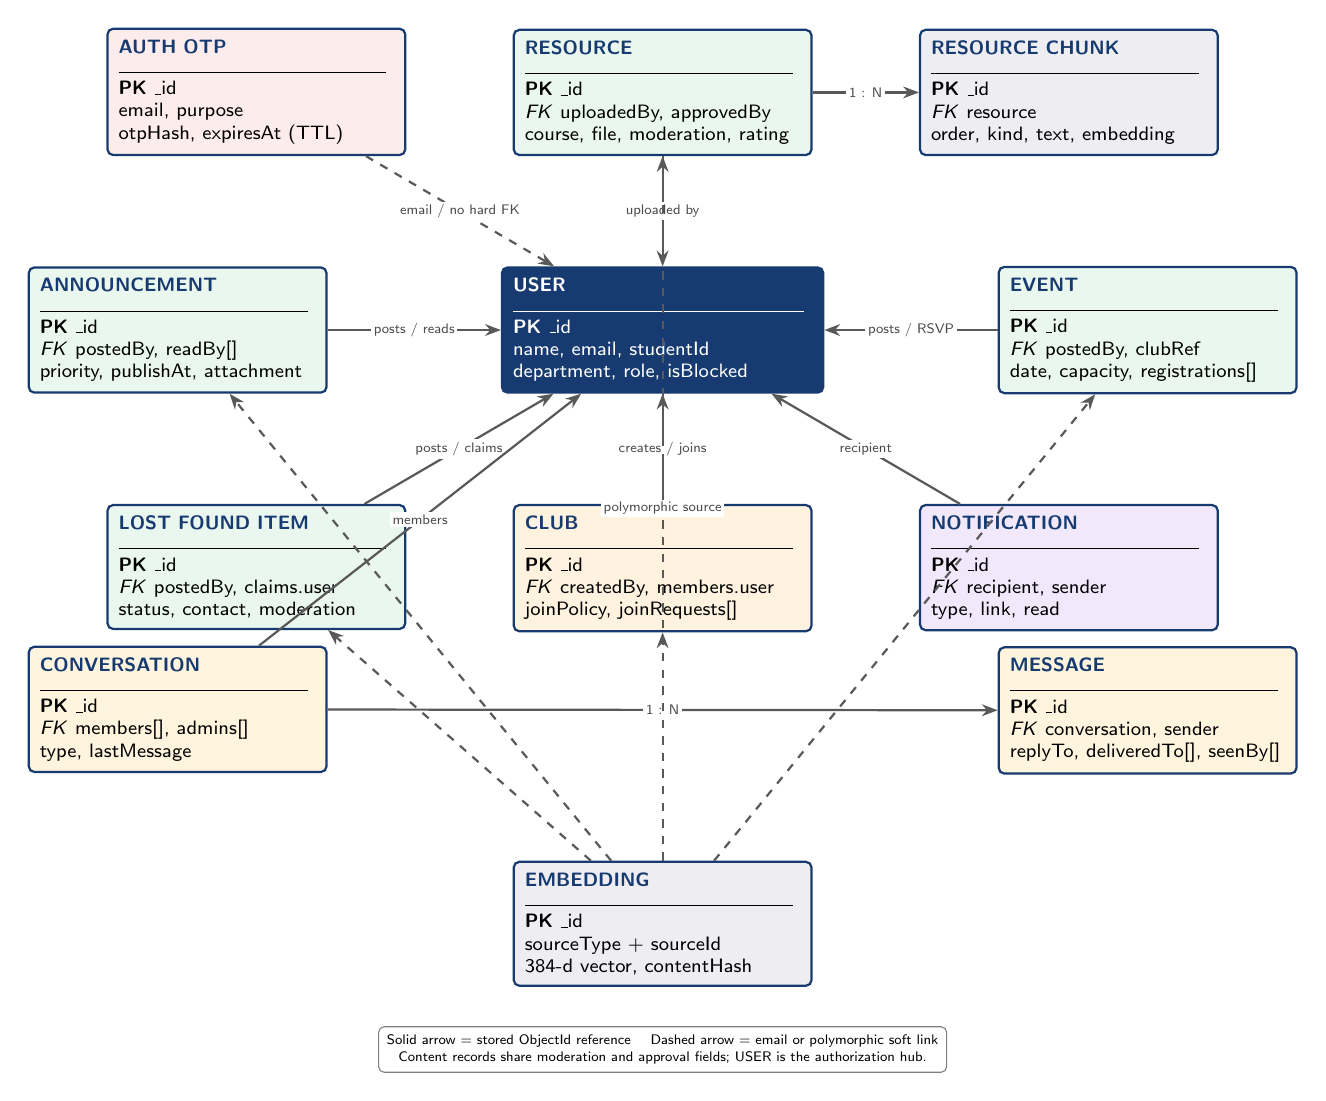
\begin{tikzpicture}[node distance=9mm and 12mm]
  \node[entity,fill=navy,text=white,text width=38mm] (user) {
    \textbf{USER}\\[-1pt]\rule{37mm}{0.3pt}\\
    \textbf{PK} \_id\\name, email, studentId\\department, role, isBlocked};

  \node[secureentity,above left=14mm and 12mm of user] (otp) {
    \entitytitle{AUTH OTP}\textbf{PK} \_id\\email, purpose\\otpHash, expiresAt (TTL)};
  \node[contententity,above=14mm of user] (resource) {
    \entitytitle{RESOURCE}\textbf{PK} \_id\\\textit{FK} uploadedBy, approvedBy\\course, file, moderation, rating};
  \node[aientity,above right=14mm and 12mm of user] (chunk) {
    \entitytitle{RESOURCE CHUNK}\textbf{PK} \_id\\\textit{FK} resource\\order, kind, text, embedding};

  \node[contententity,left=22mm of user] (announcement) {
    \entitytitle{ANNOUNCEMENT}\textbf{PK} \_id\\\textit{FK} postedBy, readBy[]\\priority, publishAt, attachment};
  \node[contententity,right=22mm of user] (event) {
    \entitytitle{EVENT}\textbf{PK} \_id\\\textit{FK} postedBy, clubRef\\date, capacity, registrations[]};

  \node[contententity,below left=14mm and 12mm of user] (lost) {
    \entitytitle{LOST FOUND ITEM}\textbf{PK} \_id\\\textit{FK} postedBy, claims.user\\status, contact, moderation};
  \node[entity,below=14mm of user,fill={rgb,255:red,255;green,243;blue,224}] (club) {
    \entitytitle{CLUB}\textbf{PK} \_id\\\textit{FK} createdBy, members.user\\joinPolicy, joinRequests[]};
  \node[entity,below right=14mm and 12mm of user,fill={rgb,255:red,242;green,232;blue,252}] (notification) {
    \entitytitle{NOTIFICATION}\textbf{PK} \_id\\\textit{FK} recipient, sender\\type, link, read};

  \node[chatentity,below=32mm of announcement] (conversation) {
    \entitytitle{CONVERSATION}\textbf{PK} \_id\\\textit{FK} members[], admins[]\\type, lastMessage};
  \node[chatentity,below=32mm of event] (message) {
    \entitytitle{MESSAGE}\textbf{PK} \_id\\\textit{FK} conversation, sender\\replyTo, deliveredTo[], seenBy[]};
  \node[aientity,below=29mm of club] (embedding) {
    \entitytitle{EMBEDDING}\textbf{PK} \_id\\sourceType + sourceId\\384-d vector, contentHash};

  \draw[soft] (otp) -- node[label]{email / no hard FK} (user);
  \draw[rel] (resource) -- node[label]{uploaded by} (user);
  \draw[rel] (resource) -- node[label]{1 : N} (chunk);
  \draw[rel] (announcement) -- node[label]{posts / reads} (user);
  \draw[rel] (event) -- node[label]{posts / RSVP} (user);
  \draw[rel] (lost) -- node[label]{posts / claims} (user);
  \draw[rel] (club) -- node[label]{creates / joins} (user);
  \draw[rel] (notification) -- node[label]{recipient} (user);
  \draw[rel] (conversation) -- node[label]{members} (user);
  \draw[rel] (conversation) -- node[label]{1 : N} (message);
  \draw[soft] (embedding) -- node[label]{polymorphic source} (resource);
  \draw[soft] (embedding) -- (announcement);
  \draw[soft] (embedding) -- (event);
  \draw[soft] (embedding) -- (lost);
  \draw[soft] (embedding) -- (club);

  \node[draw=black!50,rounded corners=2pt,below=5mm of embedding,
    font=\sffamily\tiny,align=center,inner sep=3pt] {
    Solid arrow = stored ObjectId reference \quad Dashed arrow = email or polymorphic soft link\\
    Content records share moderation and approval fields; USER is the authorization hub.};
\end{tikzpicture}
\end{document}
